\documentclass[11pt]{article}
\usepackage[utf8]{inputenc}
\usepackage[T1]{fontenc}
\usepackage{amsmath}
\usepackage{amssymb} % Needed for \eth
\usepackage{graphicx}
\usepackage{geometry}
\usepackage{tikz}
\usepackage{pgfplots} % For plots
\usepackage{ulem}     % For underline, using normalem to avoid messing with \emph
\usepackage{booktabs} % For the table

\geometry{a4paper, margin=1in}
\usetikzlibrary{positioning, arrows.meta, shapes.geometric} % For TikZ diagrams
\pgfplotsset{compat=1.18} % Use a recent PGFPlots version
\usetikzlibrary{calc} 
% Custom commands (optional)
\newcommand{\avg}[1]{\overline{#1}}
\newcommand{\prob}[1]{P(#1)}
\newcommand{\ProbDens}[1]{\mathcal{P}(#1)} % Using script P for density
\newcommand{\vect}[1]{\vec{#1}}
\newcommand{\dd}[1]{\mathrm{d}#1} % Differential d
\newcommand{\pderiv}[2]{\frac{\partial #1}{\partial #2}}
\newcommand{\deriv}[2]{\frac{\mathrm{d} #1}{\mathrm{d} #2}}
\newcommand{\muState}{\mu\text{-state}} % Microstate
\newcommand{\OmegaE}{\Omega(E)}
\newcommand{\omegaE}{\omega(E)}
\newcommand{\PhiE}{\Phi(E)}
\newcommand{\deltaE}{\delta E}
\newcommand{\ethbar}{\text{\it{đ}}} % \eth symbol for inexact differential
\newcommand{\kb}{k_B} % Boltzmann constant
\newcommand{\gasR}{R} % Ideal gas constant

\title{Physics 415 - Lecture 13: Thermodynamic Potentials and Maxwell Relations}
\date{February 19, 2025}
\author{} % Author not specified

\begin{document}

\maketitle
\thispagestyle{empty}

\section*{Summary}

Thermodynamic Potentials:
\begin{center}
\begin{tabular}{llll}
\toprule
Potential & Symbol & Natural Variables & Differential Form \\
\midrule
Internal Energy & $E$ & $E=E(S,V)$ & $dE = TdS - pdV$ \\
Enthalpy & $H=E+pV$ & $H=H(S,p)$ & $dH = TdS + Vdp$ \\
Helmholtz Free Energy & $F=E-TS$ & $F=F(T,V)$ & $dF = -SdT - pdV$ \\
Gibbs Free Energy & $G=E-TS+pV$ & $G=G(T,p)$ & $dG = -SdT + Vdp$ \\
\bottomrule
\end{tabular}
\end{center}

\section*{Equilibrium Conditions (General)}

For a closed, isolated system, equilibrium corresponds to maximum entropy $S$. Spontaneous processes lead to $\Delta S \ge 0$.

What about systems that are not closed/isolated, i.e., can exchange heat with, or do work on, their environment?

\subsection*{System at Constant T, V}

Consider system A in contact with a heat bath A' (much larger system) that maintains A at constant temperature $T$. Assume the volume $V$ of system A is also held constant (so $W=0$).

\begin{center}
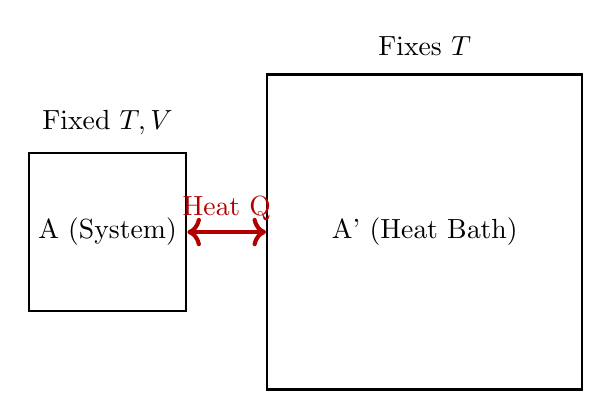
\begin{tikzpicture}
    \node (A) [draw, thick, minimum width=2cm, minimum height=2cm, label=center:A (System)] {};
    \node (Aprime) [draw, thick, minimum width=4cm, minimum height=4cm, right=1cm of A, label=center:A' (Heat Bath)] {};
    % Interface allowing heat exchange
    \draw [line width=1.5pt, red!70!black, <->] (A.east) -- (Aprime.west) node [midway, above] {Heat Q};
    % Labels
    \node at (A.north) [above=0.1cm] {Fixed $T, V$};
    \node at (Aprime.north) [above=0.1cm] {Fixes $T$};
\end{tikzpicture}
\end{center}

The total system (A+A') is isolated, so its total entropy change must satisfy $\Delta S_{tot} = \Delta S_A + \Delta S_{A'} \ge 0$.
Let $Q$ be the heat absorbed by A from the heat bath. Then the heat bath loses heat $Q$, and its entropy changes by $\Delta S_{A'} = -Q/T$ (assuming the bath process is reversible).
So, $\Delta S_A - Q/T \ge 0$, or $T \Delta S_A - Q \ge 0$.
From the First Law applied to system A: $\Delta E_A = Q - W$. Since $V$ is constant, $W=0$, so $Q = \Delta E_A$.
Substituting $Q$: $T \Delta S_A - \Delta E_A \ge 0$.
Recall the Helmholtz Free Energy $F_A = E_A - TS_A$. For a process at constant $T$, $\Delta F_A = \Delta E_A - T \Delta S_A$.
The condition $T \Delta S_A - \Delta E_A \ge 0$ is equivalent to $-\Delta F_A \ge 0$, or:
\[ \Delta F_A \le 0 \]
For a system maintained at constant temperature $T$ and constant volume $V$, the Helmholtz free energy $F$ decreases during any spontaneous process and is minimized at equilibrium. ($F=\text{min}$ in equilibrium is a consequence of $S_{tot}=\text{max}$).

\textbf{Example:} Two subsystems 1, 2 at same T, separated by movable piston, total volume $V=V_1+V_2$ fixed.
$F_{tot} = F_1(T,V_1) + F_2(T,V_2)$. Equilibrium $\implies \delta F_{tot} = 0$ for variation $\delta V_1 = -\delta V_2$.
$\delta F_{tot} = (\partial F_1/\partial V_1)_T \delta V_1 + (\partial F_2/\partial V_2)_T \delta V_2 = (-p_1)\delta V_1 + (-p_2)(-\delta V_1) = (p_2-p_1)\delta V_1$.
$\delta F_{tot} = 0 \implies p_1 = p_2$. Mechanical equilibrium required.

\subsection*{System at Constant T, p}

Consider system A maintained at constant temperature $T$ (via heat bath) and constant pressure $p$ (via piston connected to pressure reservoir).

\begin{center}
\begin{tikzpicture}
    \node (A) [draw, thick, minimum width=2cm, minimum height=2cm, label=center:A (System)] {};
    \node (Env) [draw, thick, dashed, minimum width=4cm, minimum height=4cm, right=1cm of A, label=center:Environment (Fixes T, p)] {};
    % Interface allowing heat exchange & work
    \draw [line width=1.5pt, red!70!black, <->] (A.east) -- (Env.west) node [midway, above] {Heat Q};
    \draw [line width=1.5pt, blue!70!black, <->] ($(A.east)+(0, -0.5)$) -- ($(Env.west)+(0, -0.5)$) node [midway, below] {Work W=$p\Delta V$};
    % Labels
    \node at (A.north) [above=0.1cm] {Fixed $T, p$};
\end{tikzpicture}
\end{center}

Total entropy change $\Delta S_{tot} = \Delta S_A + \Delta S_{env} \ge 0$.
$\Delta S_{env} = -Q/T$ (entropy change of environment due to heat transfer $Q$ to A).
$\implies \Delta S_A - Q/T \ge 0 \implies T \Delta S_A - Q \ge 0$.
First Law for A: $\Delta E_A = Q - W$. Since $p$ is constant, the work done by A is $W = p \Delta V_A$.
$Q = \Delta E_A + W = \Delta E_A + p \Delta V_A$.
Substituting $Q$ into the entropy condition:
\[ T \Delta S_A - (\Delta E_A + p \Delta V_A) \ge 0 \]
Recall the Gibbs Free Energy $G_A = E_A - TS_A + pV_A$. For a process at constant $T$ and $p$:
$\Delta G_A = \Delta E_A - T \Delta S_A + p \Delta V_A$.
The entropy condition becomes $- \Delta G_A \ge 0$, or:
\[ \Delta G_A \le 0 \]
For a system maintained at constant temperature $T$ and constant pressure $p$, the Gibbs free energy $G$ decreases during any spontaneous process and is minimized at equilibrium.

\section*{Maxwell Relations}

Use the thermodynamic potentials to derive some useful general results for macroscopic systems. The key mathematical idea is the equality of mixed second partial derivatives for any state function (potential).

\begin{enumerate}
    \item From $dE = T dS - p dV$:
    \[ T = \left(\pderiv{E}{S}\right)_V, \quad p = -\left(\pderiv{E}{V}\right)_S \]
    Equating $\pderiv[2]{E}{V \partial S} = \pderiv[2]{E}{S \partial V}$:
    \[ \pderiv{}{V} \left[ \left(\pderiv{E}{S}\right)_V \right]_S = \pderiv{}{S} \left[ \left(\pderiv{E}{V}\right)_S \right]_V \]
    \[ \implies \left( \pderiv{T}{V} \right)_S = - \left( \pderiv{p}{S} \right)_V \qquad (1) \]

    \item From $dF = -S dT - p dV$:
    \[ S = -\left(\pderiv{F}{T}\right)_V, \quad p = -\left(\pderiv{F}{V}\right)_T \]
    Equating $\pderiv[2]{F}{V \partial T} = \pderiv[2]{F}{T \partial V}$:
    \[ \pderiv{}{V} \left[ -\left(\pderiv{F}{T}\right)_V \right]_T = \pderiv{}{T} \left[ -\left(\pderiv{F}{V}\right)_T \right]_V \]
    \[ \implies \left( \pderiv{S}{V} \right)_T = \left( \pderiv{p}{T} \right)_V \qquad (2) \]

    \item From $dH = T dS + V dp$:
    \[ T = \left(\pderiv{H}{S}\right)_p, \quad V = \left(\pderiv{H}{p}\right)_S \]
    Equating $\pderiv[2]{H}{p \partial S} = \pderiv[2]{H}{S \partial p}$:
    \[ \pderiv{}{p} \left[ \left(\pderiv{H}{S}\right)_p \right]_S = \pderiv{}{S} \left[ \left(\pderiv{H}{p}\right)_S \right]_p \]
    \[ \implies \left( \pderiv{T}{p} \right)_S = \left( \pderiv{V}{S} \right)_p \qquad (3) \]

    \item From $dG = -S dT + V dp$:
    \[ S = -\left(\pderiv{G}{T}\right)_p, \quad V = \left(\pderiv{G}{p}\right)_T \]
    Equating $\pderiv[2]{G}{p \partial T} = \pderiv[2]{G}{T \partial p}$:
    \[ \pderiv{}{p} \left[ -\left(\pderiv{G}{T}\right)_p \right]_T = \pderiv{}{T} \left[ \left(\pderiv{G}{p}\right)_T \right]_p \]
    \[ \implies -\left( \pderiv{S}{p} \right)_T = \left( \pderiv{V}{T} \right)_p \qquad (4) \]
\end{enumerate}
Relations (1)-(4) are the \textbf{Maxwell Relations}. They are very useful in practice because they relate different partial derivatives involving $T, S, p, V$. They highlight the fact that these four variables are not all independent. Any one Maxwell relation can be derived from any other by change of variables.

\section*{Application: Relation Between $C_p$ and $C_V$}

What is the general relation between $C_p$ (heat capacity at constant $p$) and $C_V$ (heat capacity at constant $V$)? (For ideal gas, $C_p - C_V = \nu R$).

It is useful in practice because $C_p$ is often easier to measure experimentally (constant pressure is easier to maintain than constant volume), while $C_V$ might be easier to calculate theoretically.

We know $\ethbar Q = T dS$. So $C_V = T(\partial S/\partial T)_V$ and $C_p = T(\partial S/\partial T)_p$.
Let's start by considering $S$ as a function of $(T, V)$: $S=S(T,V)$.
\[ dS = \left(\pderiv{S}{T}\right)_V dT + \left(\pderiv{S}{V}\right)_T dV = \frac{C_V}{T} dT + \left(\pderiv{S}{V}\right)_T dV \]
Now let's consider $S$ as a function of $(T, p)$: $S=S(T,p)$.
\[ dS = \left(\pderiv{S}{T}\right)_p dT + \left(\pderiv{S}{p}\right)_T dp = \frac{C_p}{T} dT + \left(\pderiv{S}{p}\right)_T dp \]
We need to relate $dp$ to $dT$ and $dV$. Consider $p=p(T,V)$.
\[ dp = \left(\pderiv{p}{T}\right)_V dT + \left(\pderiv{p}{V}\right)_T dV \]
Substitute this into the second expression for $dS$:
\[ dS = \frac{C_p}{T} dT + \left(\pderiv{S}{p}\right)_T \left[ \left(\pderiv{p}{T}\right)_V dT + \left(\pderiv{p}{V}\right)_T dV \right] \]
Group coefficients of $dT$ and $dV$:
\[ dS = \left[ \frac{C_p}{T} + \left(\pderiv{S}{p}\right)_T \left(\pderiv{p}{T}\right)_V \right] dT + \left[ \left(\pderiv{S}{p}\right)_T \left(\pderiv{p}{V}\right)_T \right] dV \]
Now compare the coefficients of $dT$ and $dV$ in this expression with those from $dS$ based on $S(T,V)$:
\begin{itemize}
    \item Coefficient of $dT$: $\left(\pderiv{S}{T}\right)_V = \frac{C_V}{T} = \frac{C_p}{T} + \left(\pderiv{S}{p}\right)_T \left(\pderiv{p}{T}\right)_V$
    \item Coefficient of $dV$: $\left(\pderiv{S}{V}\right)_T = \left(\pderiv{S}{p}\right)_T \left(\pderiv{p}{V}\right)_T$ (This just confirms consistency).
\end{itemize}
From the coefficient of $dT$:
\[ \frac{C_p - C_V}{T} = - \left(\pderiv{S}{p}\right)_T \left(\pderiv{p}{T}\right)_V \]
\[ C_p - C_V = -T \left(\pderiv{S}{p}\right)_T \left(\pderiv{p}{T}\right)_V \]
This relates $C_p$ and $C_V$. However, the derivatives on the right are not readily measured. Use Maxwell relations and definitions of response functions to simplify.

\begin{itemize}
    \item Maxwell Relation (4): $\left(\pderiv{S}{p}\right)_T = -\left(\pderiv{V}{T}\right)_p$.
    \item Definition of thermal expansivity $\alpha_p = \frac{1}{V} (\partial V / \partial T)_p \implies (\partial V / \partial T)_p = V \alpha_p$.
    \item So, $(\partial S / \partial p)_T = - V \alpha_p$.

    \item Use the cyclic relation for partial derivatives $(\partial p / \partial T)_V (\partial T / \partial V)_p (\partial V / \partial p)_T = -1$.
    \[ \implies \left(\pderiv{p}{T}\right)_V = - \frac{(\partial V / \partial T)_p}{(\partial V / \partial p)_T} \]
    \item Definition of isothermal compressibility $K_T = -\frac{1}{V} (\partial V / \partial p)_T \implies (\partial V / \partial p)_T = -V K_T$.
    \item So, $(\partial p / \partial T)_V = - \frac{V \alpha_p}{-V K_T} = \frac{\alpha_p}{K_T}$.
\end{itemize}
Substitute these back into the expression for $C_p - C_V$:
\[ C_p - C_V = -T (-V \alpha_p) \left( \frac{\alpha_p}{K_T} \right) \]
\[ C_p - C_V = \frac{T V \alpha_p^2}{K_T} \]
This is the general thermodynamic relation between $C_p$ and $C_V$.
Since $T>0$, $V>0$, $K_T>0$ (usually, systems compress under pressure), and $\alpha_p^2 \ge 0$, we have $C_p \ge C_V$. They are equal only if $\alpha_p=0$ (e.g., water at 4 $^\circ$C).

\end{document}